\documentclass{beamer}

\title[Interfaz Visual de Sistemas de Ecuaciones Lineales]{Interfaz Visual de Sistemas de Ecuaciones Lineales \\ Utilizando el Método Matricial y Implementación del Framework "FLASK"}

\author[Mario Wilfredo Ramirez Puma]{Mario Wilfredo Ramirez Puma}

\institute[Universidad Nacional del Altiplano Puno]{ Universidad Nacional del Altiplano Puno \\ Escuela Profesional de Ingeniería Estadística e Informática}

\date[Mayo 2025]{Mayo 2025}

\begin{document}

% Primera diapositiva (Carátula)
\begin{frame}[plain]
    \titlepage
    \vfill
    \begin{center}
        \large \textbf{Docente: Ing. TORRES CRUZ FRED}
    \end{center}
\end{frame}

% Segunda diapositiva (Introducción)
\begin{frame}
    \frametitle{Introducción}
    La presente aplicación fue desarrollada para facilitar la resolución de sistemas de ecuaciones lineales mediante el uso del método matricial. 

    \vspace{0.5cm}

    El usuario debe ingresar el número de incógnitas del sistema. Luego, el sistema solicita los coeficientes de las ecuaciones (matriz de coeficientes) y los términos independientes. 

    \vspace{0.5cm}

    Como se trabaja con matrices cuadradas, el número de ecuaciones debe coincidir con el número de incógnitas. 

    Por ejemplo, si el sistema tiene 2 incógnitas, se requieren 2 ecuaciones. Esto implica una matriz de coeficientes de tamaño 2×2 (es decir, 4 coeficientes en total) y un vector de 2 términos independientes.

    \vspace{0.5cm}

    Esta implementación permite resolver problemas numéricos de manera sistemática y visual.
\end{frame}

\begin{frame}
    \frametitle{¿Qué es Flask?}

    Flask es un microframework para el desarrollo de aplicaciones web en Python. Es ligero, flexible y muy fácil de usar, ideal para proyectos pequeños o medianos.

    \vspace{0.5cm}
    \textbf{¿Cómo funciona?}
    \begin{itemize}
        \item Flask permite definir rutas (URLs) que responden a peticiones del navegador.
        \item Cada ruta puede procesar datos, conectarse con bases de datos, y devolver una respuesta.
    \end{itemize}

    \vspace{0.3cm}
    \textbf{Ventajas:}
    \begin{itemize}
        \item Flexibilidad total en la estructura del proyecto.
        \item Integración sencilla con HTML, CSS, JS y bases de datos.
    \end{itemize}

    \vspace{0.3cm}
    \textbf{Desventajas:}
    \begin{itemize}
        \item No incluye herramientas por defecto (como autenticación).
        \item No es ideal para proyectos muy grandes sin una buena arquitectura.
    \end{itemize}
\end{frame}

\begin{frame}
    \frametitle{Estructura de flask}
    \begin{center}
        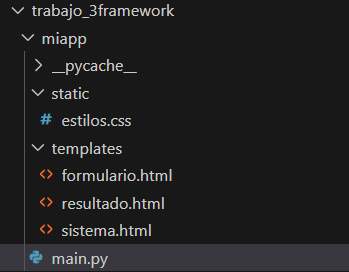
\includegraphics[width=0.8\textwidth]{cuatro.png}
    \end{center}
\end{frame}

\begin{frame}
  \frametitle{Estructura Interna de Flask}
  Flask es un microframework flexible y sencillo. No requiere una estructura rígida, pero aquí hay una estructura básica:

  \begin{itemize}
    \item \textbf{Creación de la aplicación}: Instancia de la clase Flask.
    \item \textbf{Rutas}: Se definen con el decorador \texttt{@app.route()}. Ejemplo:
    \begin{itemize}
      \item \texttt{@app.route('/')} - Función \texttt{home()}
    \end{itemize}
    \item \textbf{Plantillas (Jinja2)}: Renderizado dinámico de HTML.
    \item \textbf{Archivos Estáticos}: CSS, JS, imágenes en \texttt{static/}.
    \item \textbf{Peticiones y Respuestas}: Usando \texttt{request} y \texttt{response}.
    \item \textbf{Configuración}: Usar \texttt{config.py} para configuraciones como \texttt{SECRET\_KEY}.
    \item \textbf{Extensiones}: Como \texttt{Flask-SQLAlchemy}, \texttt{Flask-WTF}, \texttt{Flask-Login}.
  \end{itemize}
\end{frame}

\begin{frame}
    \frametitle{Vista de Ecuaciones}
    \begin{center}
        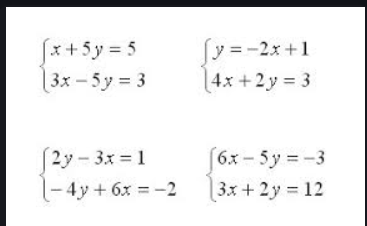
\includegraphics[width=0.8\textwidth]{cero.png}
    \end{center}
\end{frame}

\begin{frame}
    \frametitle{Interfaz de Entrada de Datos}
    \begin{center}
        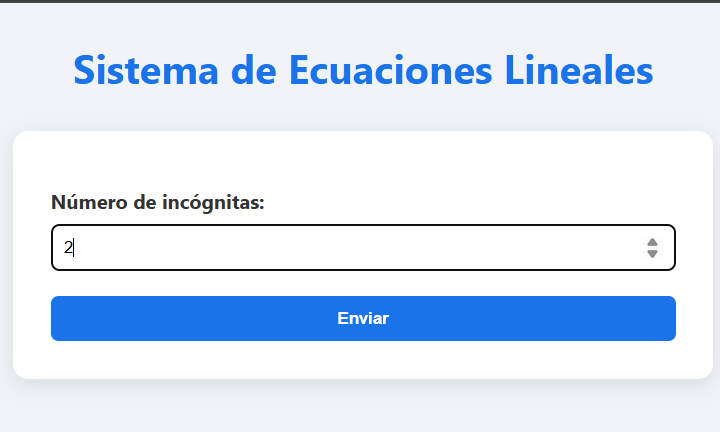
\includegraphics[width=0.8\textwidth]{primer.png}
    \end{center}
\end{frame}

\begin{frame}
    \frametitle{Coeficientes y Terminos Independientes }
    \begin{center}
        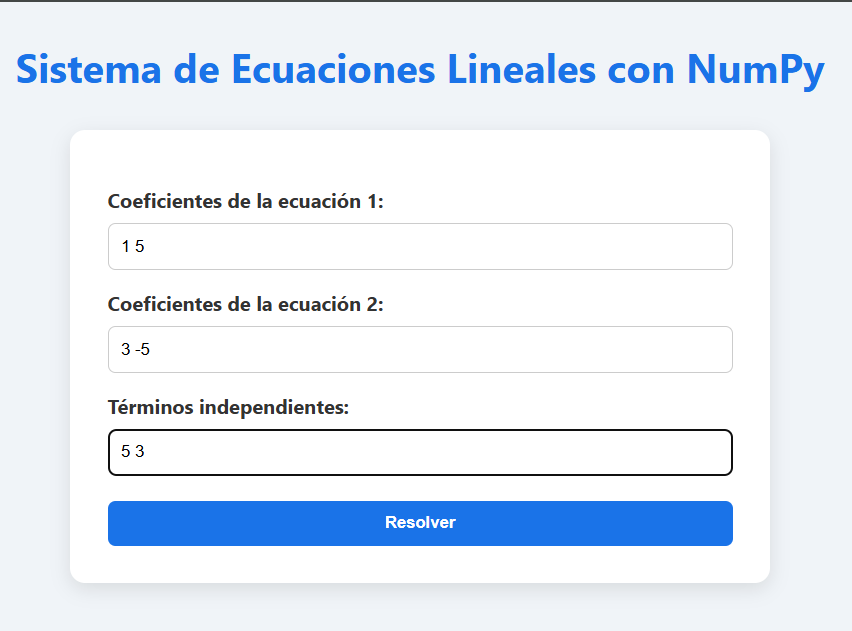
\includegraphics[width=0.8\textwidth]{segundo.png}
    \end{center}
\end{frame}

\begin{frame}
    \frametitle{Salida}
    \begin{center}
        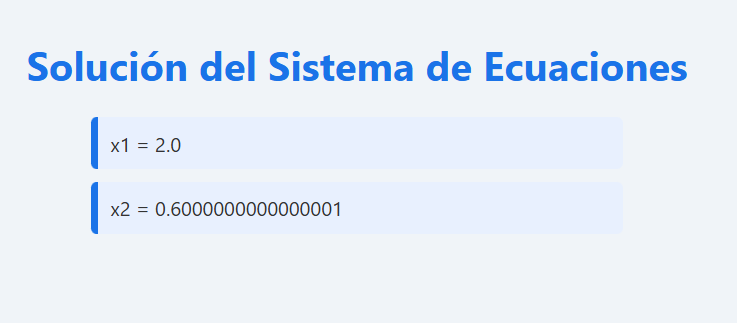
\includegraphics[width=0.8\textwidth]{tercero.png}
    \end{center}
\end{frame}

\begin{frame}
    \frametitle{}
    \begin{center}
        \huge \textbf{¡Gracias por tu atención!}
    \end{center}
\end{frame}

\end{document}
